\section{Reconfigurable Hardware}
A significant portion of the project's work involves exploiting reconfigurable hardware to vastly reduce the inference time of the proposed neural networks. This section explains in more detail the technology and characteristics of reconfigurable hardware, and in particular, FPGAs.

\subsection{Landscape of Hardware for Computing}
The modern landscape of digital integrated circuits (IC) is very rich can be divided into numerous categories depending on the technology used and expected functionality \cite{14-najafi2017hardware}. A list of platform types is described below, with the emphasis of their suitability for neural networks applications.

\begin{itemize}
  \item \textbf{Central Processing Units (CPU)} - the most commonly found ICs that are at the core of personal computers, laptops and handheld devices. They are capable of executing a broad range of predefined instructions. As CPUs have become widely adopted in research long before the emergence of the other technologies from this list, they were the first platforms for the training and inference of neural networks with promising results back in the 1980s and 1990s for applications like high energy physics \cite{17-dagli1989applications} or biology \cite{16-wu1995neural}. Although it is possible to achieve speed-ups of over 10x the baseline performance with careful optimizations \cite{nn_cpu_optim}, CPUs are now consistently outperformed by more suitable technologies, and only limited to certain inference tasks.

  \item \textbf{Graphic Processors (GPU)} - ICs originally specialized in graphics processing intended for displaying images. Since their inception, due to the type of calculations involving matrix and vector operations, other applications related to cryptography and neural networks have also adopted GPUs as their main platform. In the former domain, cryptocurrency mining has transitioned from CPU to GPU to increase profitability \cite{19-iyer2018gpu}, while for the latter, the more powerful hardware drastically reduced training and inference times, thus allowing for deeper and more complex architectures yielding higher accuracy \cite{20-chen2020gpu-accelerated, 21-zhang2019recent}.

  \item \textbf{Application Specific Integrated Circuits (ASIC)} - as suggested by the name, those are the custom designed ICs heavily specialized for a particular application. It is hard to generalize them, as the use cases can cover any modern computing problem, but the commonality is a vast improvement in performance and power usage compared to more general purpose solutions. However, the long and expensive development process pose extremely high barriers to entry for most users. Fortunately, off-the-shelf products like the Graphcore Intelligence Processing Units \cite{22-graphcoregraphcore}, that are designed specifically with machine learning applications in mind, as well as other custom designs \cite{23-knag2015sparse, 24-ramanaiah2011asic} are starting to offer a compelling platform for working with neural networks.

  \item \textbf{Field-Programmable Gate Arrays (FPGA)} - differently from the previous listed IC types, FPGAs are not manufactured for a specific use case, and in fact, they can be reprogrammed to be a platform for a different application at any time. The reprogrammability comes at a cost of performance and power consumption compared to ASICs \cite{25-boutros2018improve}, but at the same time outperforms GPUs in these regards \cite{27-nurvitadhi2017fpgas, 28-li2018gpu-outperforming}. It is also suggested, that with some technological improvements focused on ML applications, FPGAs can narrow the gap between ASICs without needing to stick to one particular design \cite{25-boutros2018improve, 26-nurvitadhi2016accelerating, 15-nurvitadhi2016accelerating}.

\end{itemize}

FPGAs offer an interesting trade-off between implementation effort and acceleration potential when it comes to neural networks and for that reason they have been chosen as the target technology in this report. The following subsections give a closer look at some of their characteristics and associated tools.

\todofig{FPGA lattice overview to visualize explain the idea behind this technology}
\todofig{|}
\todofig{|}
\todofig{|}

\subsection{High-Level Synthesis}
For many years, FPGAs have been modelled using register-transfer level (RTL) design abstraction with the use of hardware description languages like Verilog or VHDL. However, to increase productivity and allow for a more convenient design state space exploration (DSE), a more abstract modelling process called High-Level Synthesis (HLS) can be adopted. The design can be expressed in a software programming language like C, C++ or Java, which can be both manually and automatically optimized, and transformed to an equivalent RTL. This is especially beneficial in research, where compared to industrial environment, it is more likely that a slightly lower quality of results can be afforded for increased productivity and easier DSE. In fact, a recent study shows that on average only one third of design time and half of the lines of code are needed for an equivalent project done in HLS in comparison to RTL while the quality of results varies and can even outperform the RTL implementations for some applications \cite{30-lahti2019yet?}.

This report's work is based on Xilinx Vivado HLS design suite. When developing a solution, it is important to note, that the synthesis process can take a significant amount of time (from a couple of hours to days on a modern powerful machine), and so there exist two simulation methods - a C-simulation that can quickly and directly evaluate a software benchmark against an emulation of the design, and a more truthful, cosimulation that firstly synthesizes a design and accompanying test bench to RTL and then performs an RTL simulation. A final, definitive evaluation of the results requires programming a target FPGA with the generated bit stream of the design and exchanging input/output data with a program that usually runs on a CPU.

\todofig{HLS to RTL flow diagram}
\todofig{|}
\todofig{|}
\todofig{|}


\subsection{\hlsml Codesign Workflow}
A commonality between the recent best performing hardware-mapped neural network models is the use of the \textit{hls4ml} codesign workflow that was mentioned in \cref{motivation}.
\indo{More about hls4ml}
\indo{Difficulty: rtl > hls > python hl4ml, draw comparison with assembly}
\indo{|}
\indo{|}
\indo{|}
\indo{|}


\subsection{Latency, Throughput, and Hardware Resources}\label{latency-throughput-resources}
To properly navigate during the DSE and assign scores the solutions, the following characteristics have to be considered:

\begin{itemize}
  \item \textbf{Latency} - A time measure of a system between receiving an input signal and producing a \textit{corresponding} output. It is crucial in real-time processing where it has to be lower than the period between subsequent input samples. Depending on the application, latency in the microseconds or nanoseconds range can be expected from an FPGA. To recall from \cref{triggers}, the latency constraint for this work comes from the specification of L1T at LHC and is equal to \(12.5\; \mu s\).
  \item \textbf{Throughput} - A rate of samples processed in a unit of time. For architectures that only start to process new elements after the previous one has finished, it is directly linked to latency. However, in modern ICs, especially in FPGAs, it is one of the defining metrics of performance and designs tend to exploit pipelining and parallelizability to marginally trade off their latency to increase it. Despite that, in this work, this measure is of little interest given the fixed latency and no dead-time constraint of L1T.
  \item \textbf{Resource utilization} - A more complicated, often multidimensional, metric that describes either the raw number or ratio of total usage of the hardware components of an FPGA. Typically, the higher it becomes, the more power is drawn by an FPGA, however, it is most often used to guide the design process to avoid running out of a certain resource. This can be done by potentially deploying an alternative method that can be implemented using a different, less contested resource. 
\end{itemize}

While FPGAs vary in terms of hardware resource configurations, several key components can be distinguished:

\begin{itemize}
  \item \textbf{Block Random Access Memory (BRAM)} - RAM unit which offers higher capacity storage with a relatively high access latency. It is best for storing big chunks of data that are not continuously used.
  \item \textbf{Lookup Table (LUT)} - a simple memory component that can store a very limited number of values while offering low access latency. It is often used for storing precomputed function values which can remove complex calculations from the critical path.
  \item \textbf{Flip-Flop (FF)} - more precisely, a D flip-flop, which implements a basic 1-bit binary register.
  \item \textbf{Digital Signal Processing (DSP) slice} - a logic element that is very efficient at additions, subtractions, multiplications, and boolean logic operations. It can process more than two inputs at once, which efficiently handles common algebraic operations like multiply-accumulate.
\end{itemize}

To fully understand the trade-offs between designs, one cannot forget about the metric directly related to the specific task that is accelerated in hardware. In the case of this report, classification accuracy and AUC described in \cref{ml-accuracy-auc-confusion}, will also play key roles in evaluating various configurations.


\subsection{Serial, Parallel, and Pipelined Architectures}\label{serial-parallel-pipelined}
Hardware architectures use components that can be configured in different ways depending on the overall goal or a limiting factor. The high-level configurations of building blocks are displayed in figure \ref{fig:serial-parallel-pipelined} and can be described as follows:

\begin{itemize}
  \item \textbf{Serial} - elements are arranged in a chain, processing one after another. This way uses less resources than an equivalent parallel configuration by reusing given components \(R\) times, thus approximately trading-off \(R\) times less required resources for \(R\) times higher latency.
  \item \textbf{Parallel} - elements share a common input and start processing data at the same time. This way ends in a lower latency than an equivalent serial configuration consuming using more resources.
  \item \textbf{Pipelined} - a more sophisticated arrangement, in which subsequent processing blocks (that can be either placed serially or in parallel) form a pipeline of processing stations separated by simple storage elements called pipeline registers, implemented using FFS. This maximizes the usage of the design blocks, hence increasing throughput with a minimal sacrifice of latency and resource usage.
\end{itemize}

\begin{figure}[hpt!]
  \centering
  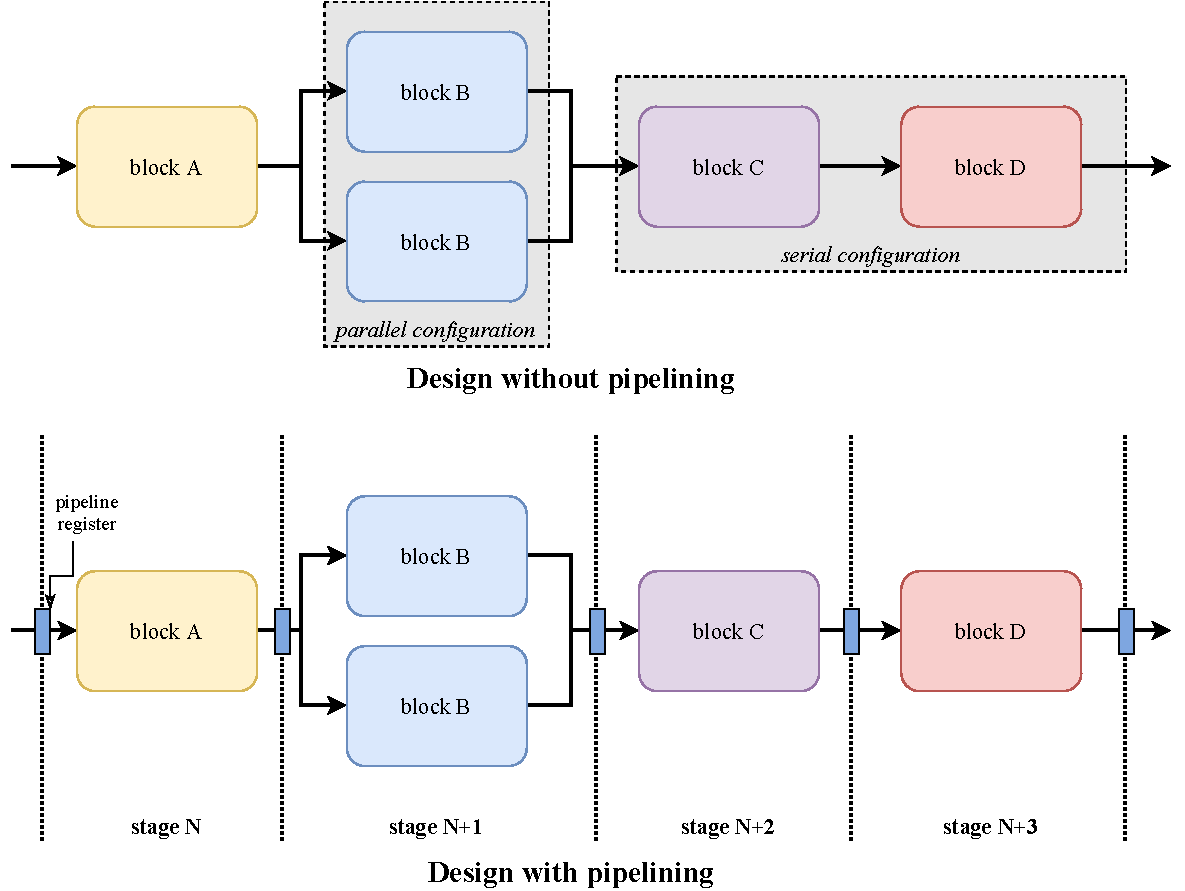
\includegraphics[trim={0cm 0cm 0cm 0cm}, width=0.75\textwidth, center]{background/serial_parallel_pipelined.pdf}
  \caption{Diagram comparing serial and parallel configurations as well as showcasing designs with and without pipelining.}
  \label{fig:serial-parallel-pipelined}
\end{figure}

\pagebreak
\subsection{Pareto Front and Roofline Model}
To make an informed design decision, various architectures can be compared by arranging them on a dependency graph (e.g. latency vs resource usage) and observing the Pareto front - the set of solutions for which there are no better ones in regard to one quality given that the other measure is not worse. The slightly complex definition can be easily understood from figure \ref{fig:pareto}, which also highlights another use of this method - finding design configurations that are yet to be explored.

\begin{figure}[hpt!]
  \centering
  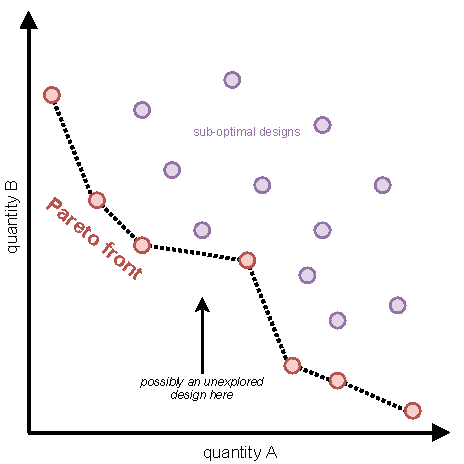
\includegraphics[trim={0cm 0cm 0cm 0cm}, width=0.5\textwidth, center]{background/pareto.pdf}
  \caption{Example graph with designs plotted against quantities A/B, Pareto front highlighted.}
  \label{fig:pareto}
\end{figure}

\pagebreak
Another intuitive performance visualization comes in the form of the Roofline model, which compares the obtained results with theoretical limits coming from inherent hardware limitations like clock frequency or memory bandwidth. An example can be seen in fig \ref{fig:roofline}.

\begin{figure}[hpt!]
  \centering
  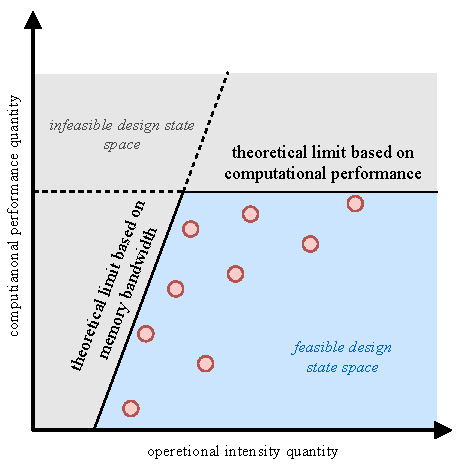
\includegraphics[trim={0cm 0cm 0cm 0cm}, width=0.5\textwidth, center]{background/roofline.pdf}
  \caption{Example graph with computational and memory bandwidth limitations showcasing the Roofline model}
  \label{fig:roofline}
\end{figure}